\documentclass{article}

\usepackage{graphicx}
\usepackage{subcaption}

\begin{document}

This is the line of text above the figure in my \LaTeX{} document.

\begin{figure}[h]
  \centering
    \begin{subfigure}[t]{0.5\textwidth}
      \centering
      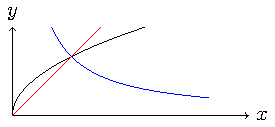
\includegraphics[width=\linewidth]{figs/example_graph.pdf}
      \caption{This is the first subfigure. This is a super long caption that will go over a single line.}\label{fig:subfig1}
    \end{subfigure}%
    \begin{subfigure}[t]{0.5\textwidth}
      \centering
      
\includegraphics[height=3cm]{figs/Snipping_tool_image.png}
      \caption{This is the second subfigure}\label{fig:subfig2}
    \end{subfigure}
  \caption{This is the figure}\label{fig:example}
\end{figure}


This is a line of text below the figure. We are talking about Figure~\ref{fig:example}. Here I refer to the first subfigure as Figure~\ref{fig:subfig1} and the second subfigure as Figure~\ref{fig:subfig2}.

\end{document}
